\documentclass[11pt]{beamer}

\usetheme{metropolis}

\usepackage{graphicx}
\usepackage{physics}
\usepackage{adjustbox}
\usepackage{caption}
\usepackage{chemformula}
\usepackage{quoting}
\usepackage[style=chem-angew,backend=bibtex]{biblatex}
\bibliography{references}
%
% Choose how your presentation looks.
%
% For more themes, color themes and font themes, see:
% http://deic.uab.es/~iblanes/beamer_gallery/index_by_theme.html
%
\mode<presentation>
{
  \usetheme{default}      % or try Darmstadt, Madrid, Warsaw, ...
  \usecolortheme{default} % or try albatross, beaver, crane, ...
  \usefonttheme{default}  % or try serif, structurebold, ...
  \setbeamertemplate{navigation symbols}{}
  \setbeamertemplate{caption}[numbered]
  \setbeamerfont{footnote}{size=\tiny}
} 

\usepackage[english]{babel}
\usepackage[utf8]{inputenc}
\graphicspath{{image/}}

\AtBeginSection[]{
\begin{frame}{Outline}
  \tableofcontents[currentsection]
\end{frame}
}

\title{Chapter 7: Electron Structure of the Atom}
\institute{Chemistry Department, Cypress College}
\date{Nov 7, 2022}

\begin{document}

\begin{frame}
  \titlepage
\end{frame}

\begin{frame}{Class Announcements}
  \textbf{Lab}
  \begin{itemize}
  \item Experiment 17 Lewis Structures and Molecular Models
  \item Basic steps for lewis structures
  \item Reminder - Need $70\%$ of laborator points to pass
    the course
  \end{itemize}

  \textbf{Lecture}
  \begin{itemize}
  \item Finish up Ch 7 and begin Ch 8
  \item Go over homework 9 (EC for students who present)
  \item Quiz and Homework assignment released Fri, Nov 11th at 3pm
  \end{itemize}
\end{frame}

\section{Review: Periodicity of Electron Configurations}

\begin{frame}{Atomic Orbitals}
  \centering
  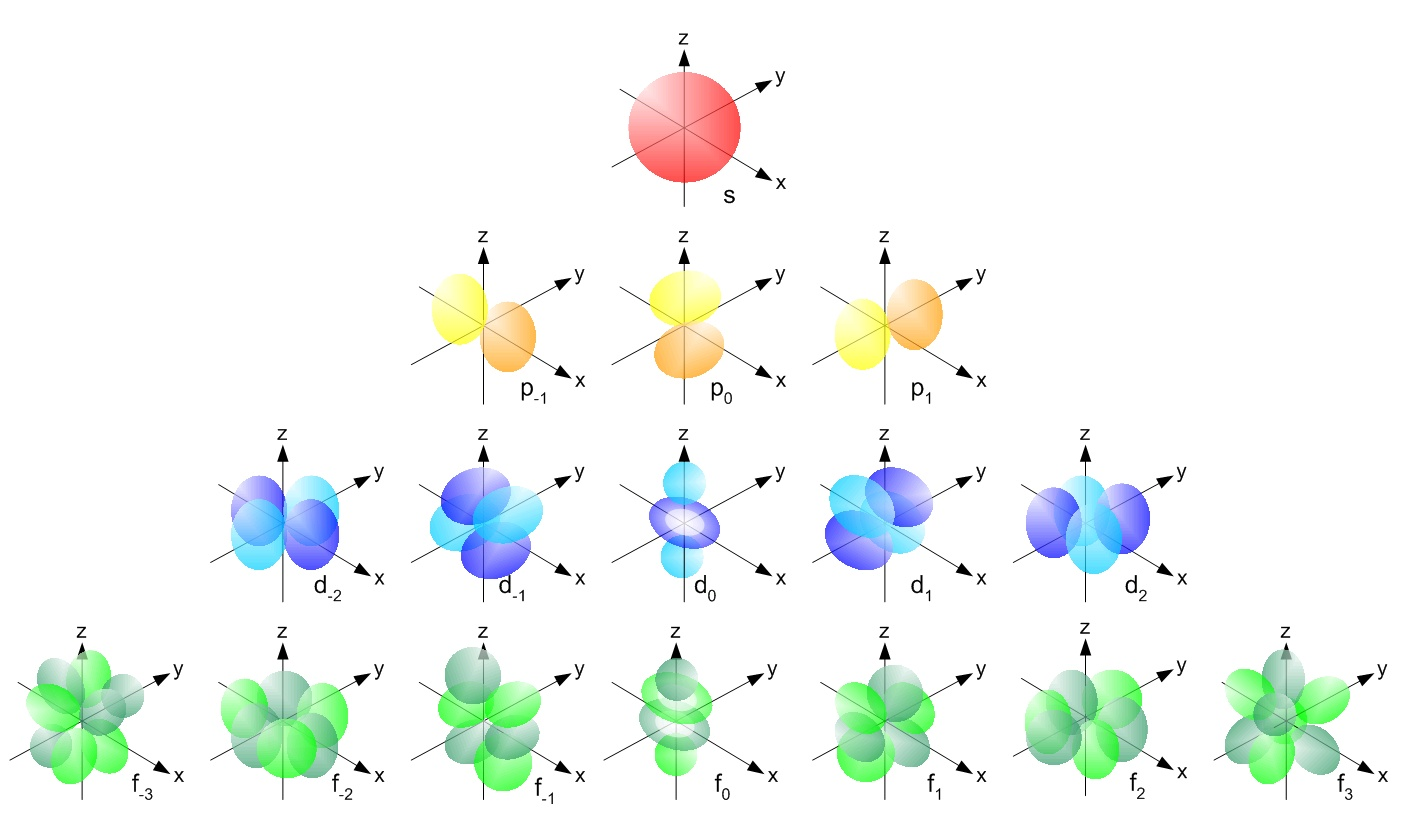
\includegraphics[width=0.8\linewidth]{single_elect_orb}
  \begin{itemize}
  \item Specific orbitals occupy certain \textbf{principal energy level} e.g.
    $n = 1, 2, 3, \cdots$
  \item Basis in which atoms form bond; atomic orbitals combine to make
    molecular orbitals
  \end{itemize}
\end{frame}

\begin{frame}{Orbital Diagram - Multielectron Element}
  \textbf{Q:} What do notice about the relative atomic orbital energies?
  
  \centering
  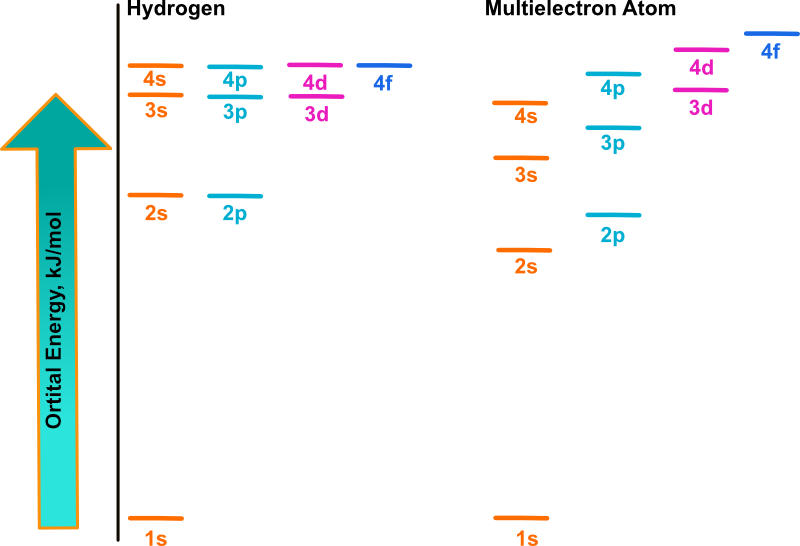
\includegraphics[scale=1.3]{orbital_energy}
\end{frame}

\begin{frame}{Principles for Filling Atomic Orbitals}
  \textbf{Aufbau principle} - electrons fill an orbital starting with
  the lowest energy level

  \textbf{Pauli exclusion princple} - No two electrons with the same
  spin can occupy the same orbital

  \textbf{Hund's Rule} - Maximize the number of unpaired electrons
\end{frame}

\begin{frame}{Relating to Periodic Table}
  \centering
  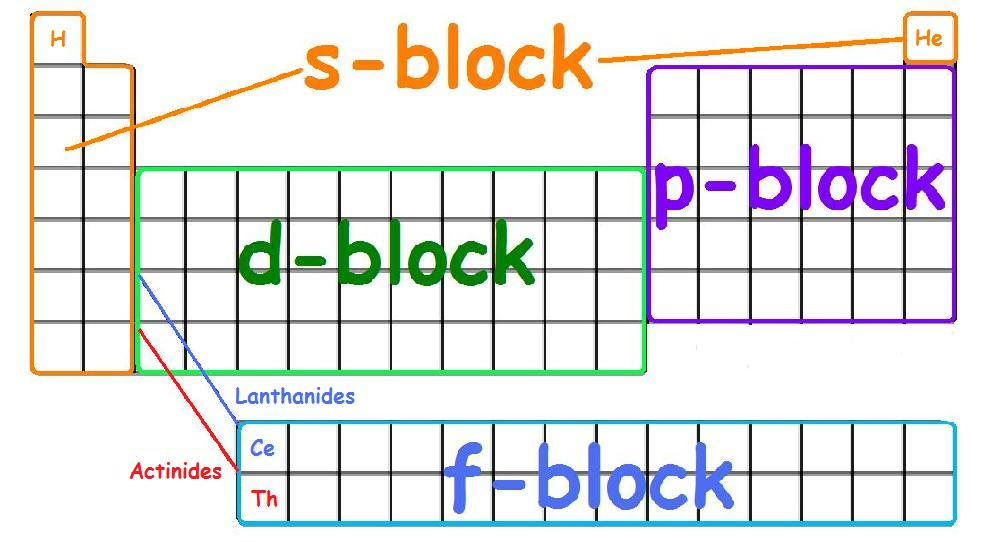
\includegraphics[width=\linewidth]{spdf_orbitals}
\end{frame}

\begin{frame}{Purpose of Electron Configurations}
  \begin{itemize}
  \item Outermost shell is referred to as the valence
    electrons (\textbf{Q:} What is special about valence electrons?)
  \item Innermost shell is the core electrons
  \item Predicts stability of the atom e.g. unfilled orbitals
    indicate instability
  \item Make predictions how elements react forming new chemical
    compounds
  \end{itemize}
\end{frame}

\section{Valence electrons for Main-Group Elements}

\begin{frame}{Core and Valence Electrons}
  \textbf{Core Electrons} - Energy level $n$ below the valence
  electrons and these are completely filled orbitals

  \textbf{Valence Electrons} - Outermost electrons above the energy
  level $n$ of the core electrons

  \textbf{Example:} Si - $1s^22s^22p^63s^22p^2$
\end{frame}

\begin{frame}{Practice: Determine number of valence electrons}
  \textbf{Au}
  \vspace{0.25in}

  \textbf{Na}
  \vspace{0.25in}
  
  \textbf{Sb}
  \vspace{0.25in}
  
  \textbf{Ag$^+$}
  \vspace{0.25in}

  \textbf{Cu$^{3+}$}
  \vspace{0.25in}

  \textbf{Ca$^{2+}$}
  \vspace{0.25in}
  
\end{frame}

\section{Periodict Properties of Atoms}

\begin{frame}{Ionization Energy}
  \textbf{Ionization energy} - Energy required to eject an electron

  \centering
  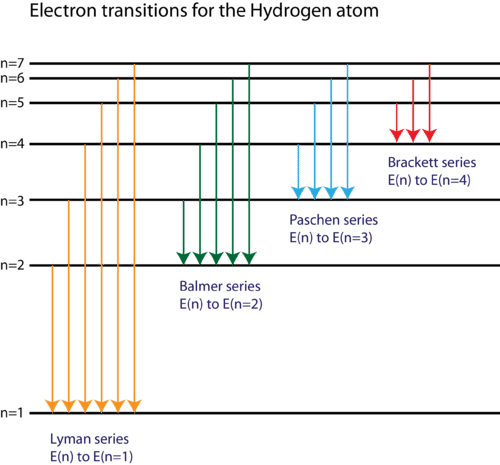
\includegraphics[scale=0.35]{energy_trans_h}
\end{frame}

\begin{frame}{Meaning of Ionization}
  \begin{center}
    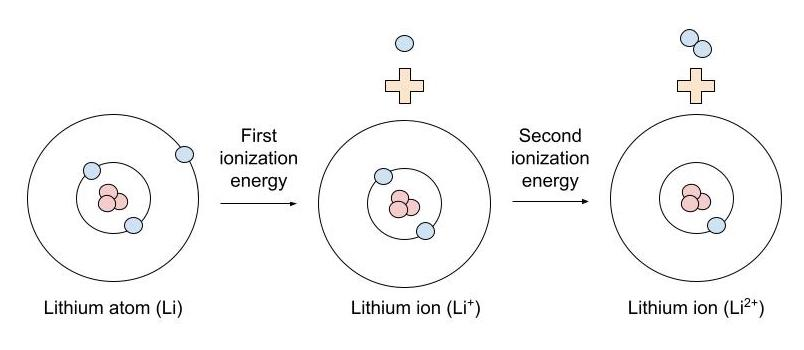
\includegraphics[width=\linewidth]{ionization_Li}
  \end{center}

  First ionization takes 520 kJ/mol and second ionization takes
  7298 kJ/mol

  \textbf{Q:} Why is the second ionization energy significantly higher?
\end{frame}

\begin{frame}{First Ionization Energy Trends}
  \centering
  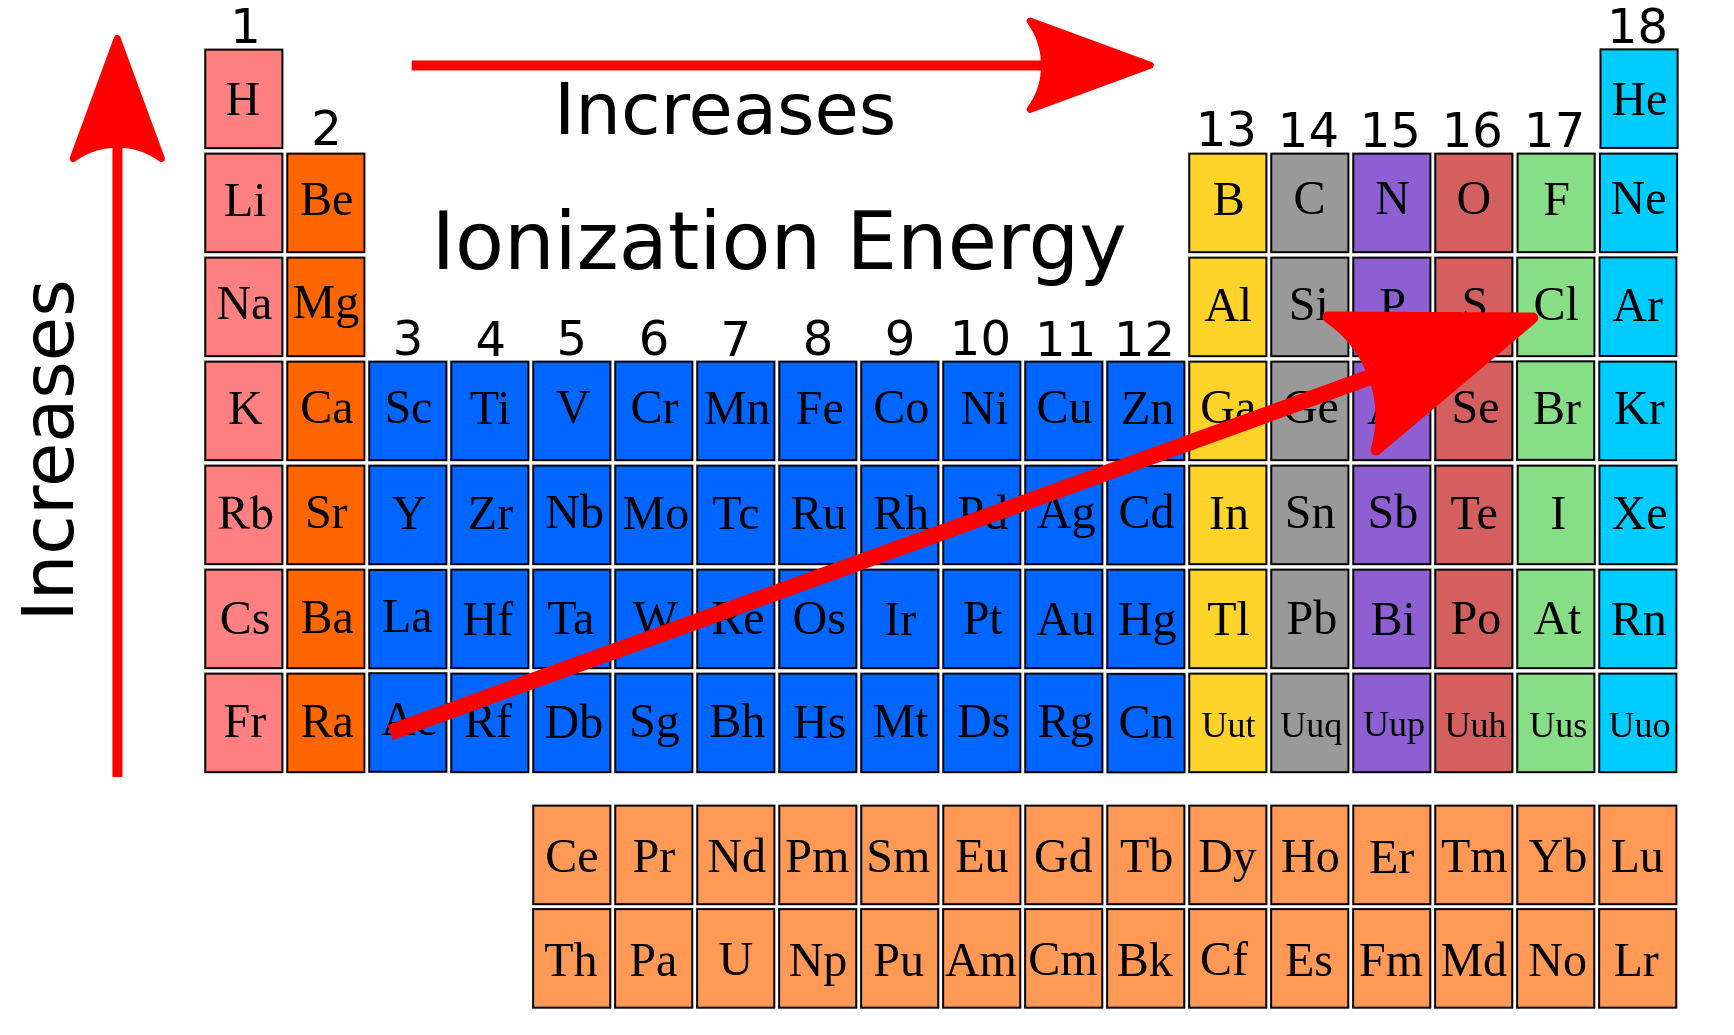
\includegraphics[width=\linewidth]{ion_trends}
\end{frame}


\begin{frame}{First Ionization Energy Trends}
  \centering
  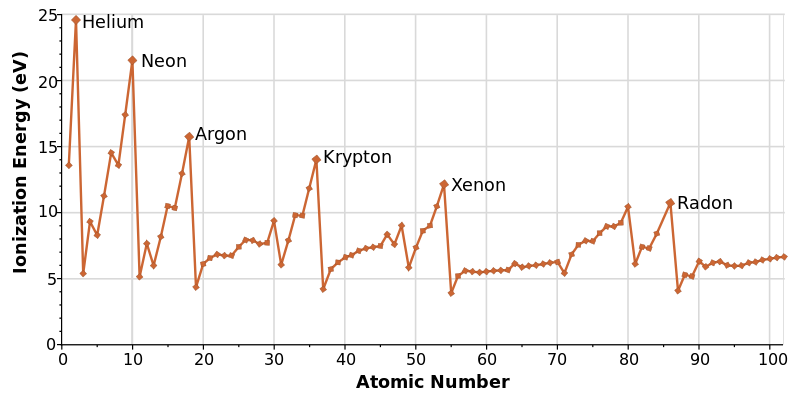
\includegraphics[width=\linewidth]{first-ionization-energy}
\end{frame}

\begin{frame}{Atomic Sizes of Neutral Atoms}
  \centering
  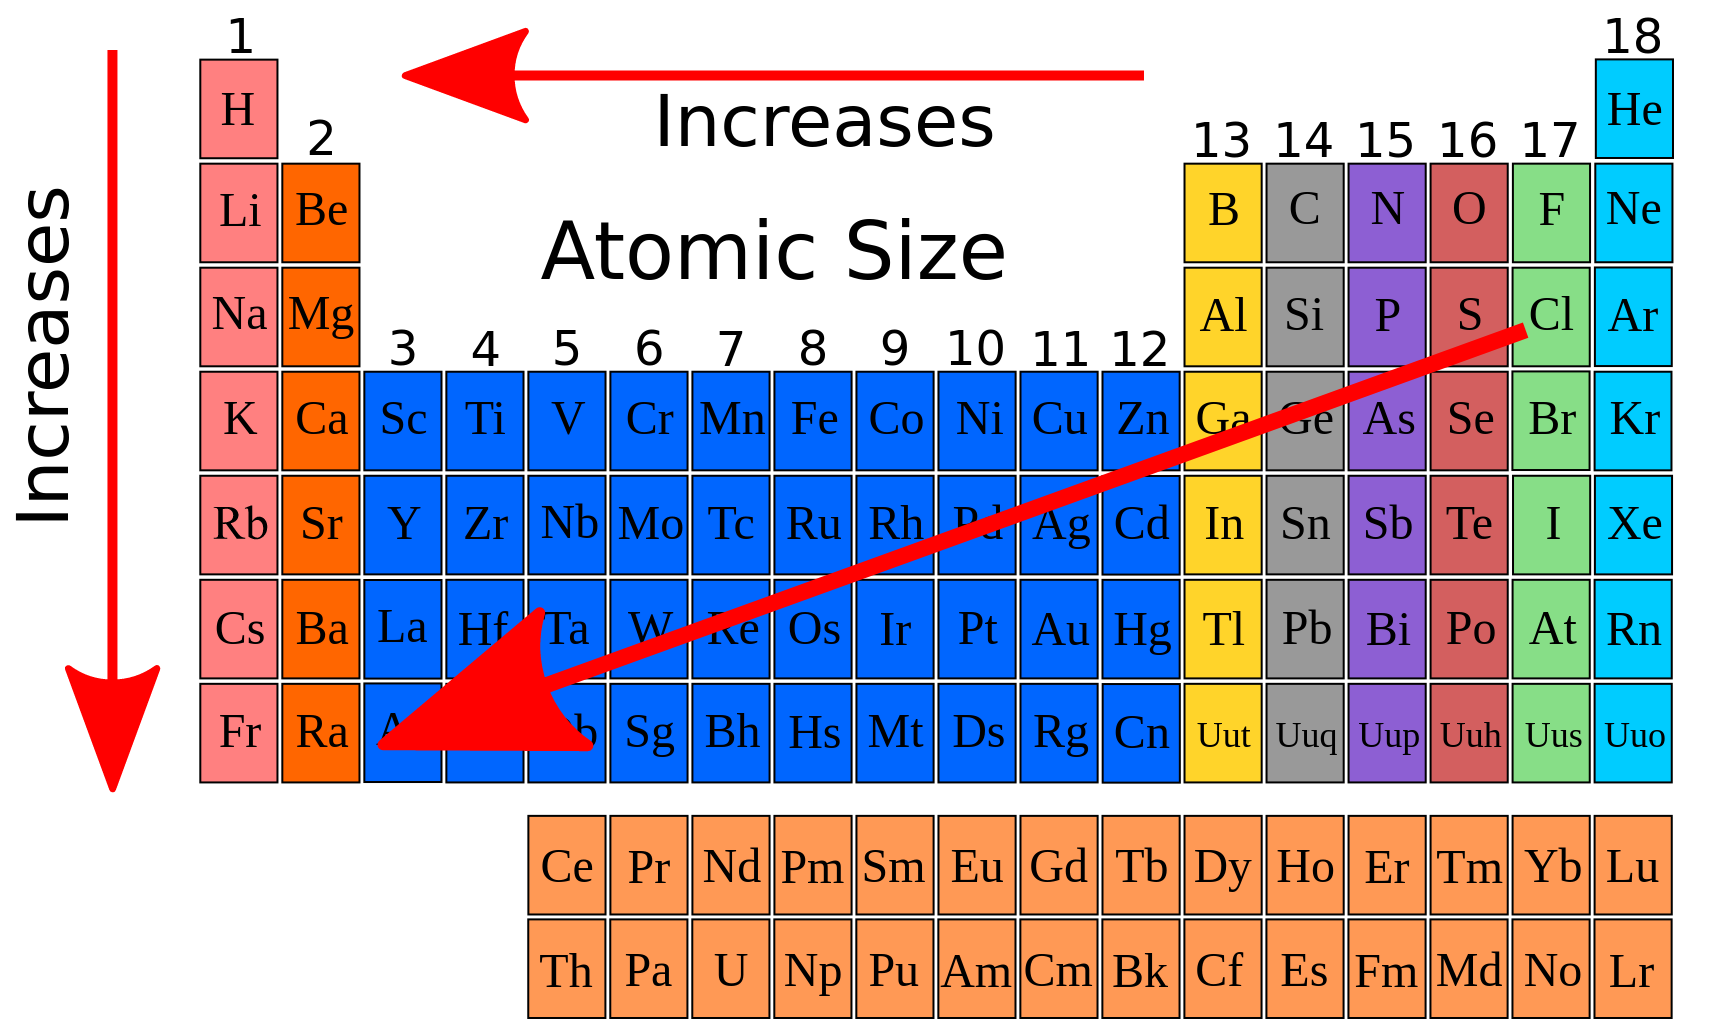
\includegraphics[width=\linewidth]{atomic_trend}
\end{frame}

\begin{frame}{Atomic Sizes of Neutral Atoms}
  \centering
  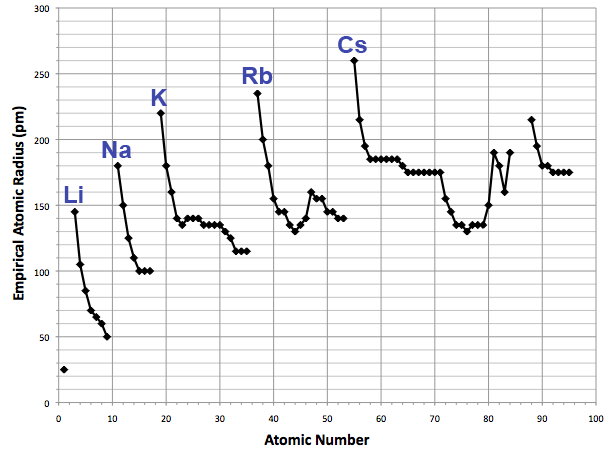
\includegraphics[width=\linewidth]{graph_atomic_rad}
\end{frame}

\begin{frame}{Atomic Sizes of Ions}
  \centering
  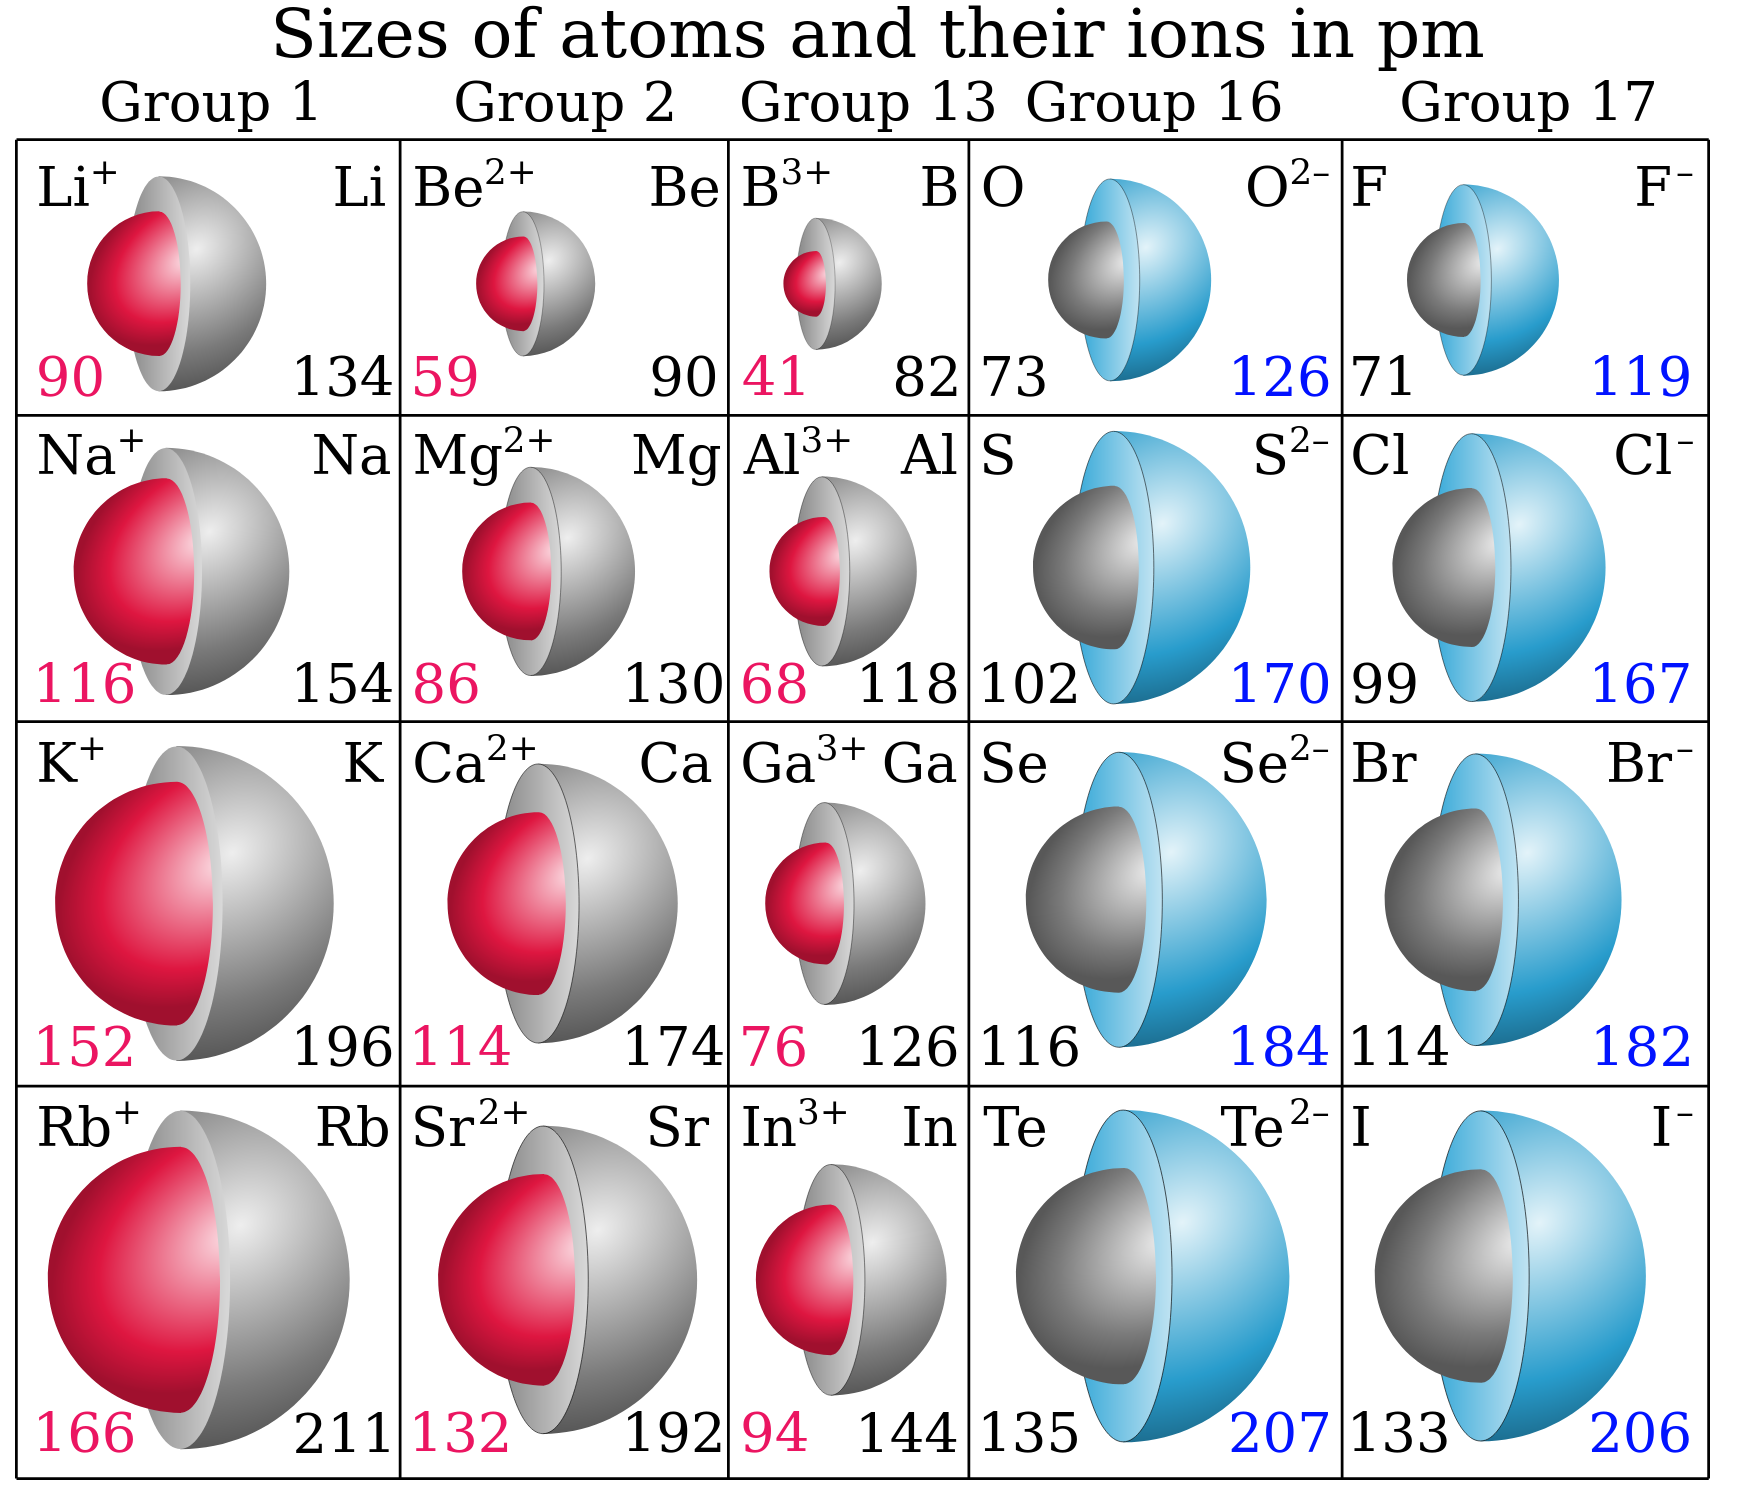
\includegraphics[width=0.8\linewidth]{ion_radii}
\end{frame}

\end{document}
